\chapter{K-módszer}

A K-módszer (Kirchoff-módszer) célja, hogy szétválassza a rendszer lineáris részét és az olyan 
részt, amelyben késleltetés nélküli út van. Ezután a késleltetés nélküli részt 
geometriai módszerekkel oldja meg.

\section{A K-módszer alapgondolata}\label{KSep}
A K-módszer alapfeltevése, hogy a modellezendő rendszer felbontható egy lineáris dinamikus és egy 
nemlineáris memória nélküli részre~\cite{borin}\cite{borin2}\cite{otherK}. 
\begin{equation}
    \begin{cases}
        \mathbf{x}(t)=\mathbf{L}(\mathbf{y}(t),\mathbf{u}(t)) \\
        \mathbf{y}(t)=\mathbf{f}_{NL}(\mathbf{x}(t)) 
    \end{cases} 
\end{equation}
Így, hogy a rendszer két részre van osztva, azokat a bemeneteket és kimeneteket fogják érinteni 
a számolási nehézségek, amelyek függenek a nemlineáris résztől.
\begin{figure}[H]
    \centering
    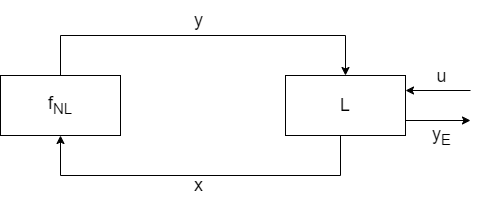
\includegraphics[scale=0.5]{figures/xy.png}
    \caption{A K-módszer alapfeltétele; $\mathbf{u}$ a bemenet, és $\mathbf{y_E}$ a kimenet a külvilág felé}
\end{figure}
Ha a rendszert a hátralépő Euler módszer, akár a bilineáris transzformáció segítségével diszkretizáljuk, akkor a következő összefüggéshez jutunk~\cite{borin}:
\begin{equation}
    \mathbf{x}[n]=\mathbf{Ky}[n]+\mathbf{p}[n]    
\end{equation}
ahol a rendszernek $M$ darab ``belső`` bemente ($y_1 \ldots y_M$), $P$ darab ``külső`` bemenete ($u_1 \ldots u_P$) és $N$ darab ``belső`` kimenete ($x_1 \ldots x_N$) van.

\begin{figure}[H]
    \centering
    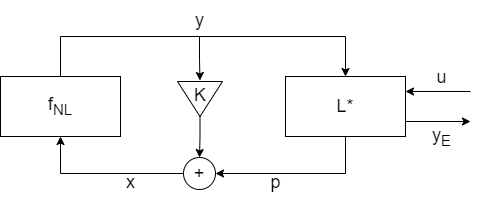
\includegraphics[scale=0.5]{figures/pxy.png}
    \caption{A rendszer felbontva; $\mathbf{L^*}$-nak az $\mathbf{y}$ bemenete és $\mathbf{p}$ kimenete között nincs késleltetés nélküli 
    összeköttetés}
\end{figure}
Ebben az összefüggésben $\mathbf{p}$ egy $\mathbf{L^*}$ rendszer kimenete, amelyet csak a definiált ($\mathbf{u}$) és a múltbéli jelek határoznak meg. 
Ekkor felírható a rendszer az alábbi formában~\cite{borin}:
\begin{equation}
    \begin{cases}
        \mathbf{p}[n]=\mathbf{L^*}(\mathbf{u}[n],\mathbf{y}[n]) \\
        \mathbf{y}[n]=\mathbf{f}_{NL}(\mathbf{p}[n]+\mathbf{Ky}[n])
    \end{cases}
\end{equation}
Fontos megjegyezni, hogy az $\mathbf{L^*}$ rendszernek nincs semmilyen késleltetés nélküli kapcsolata $\mathbf{y}$ és $\mathbf{p}$ között. 
Így a számolási probléma az $\mathbf{y}[n]=\mathbf{f}_{NL}(\mathbf{p}[n]+\mathbf{Ky}[n])$ részre korlátozódik, amely explicit megoldásához a Dini-tételt alkalmazandó, 
vagy megoldható valamelyik szokásos Newton-módszerrel.

Ha létezik $\mathbf{y}=\mathbf{g}_{NL}(\mathbf{p})$ explicit függvény és ezt meg tudjuk találni, akkor a számítási problémát ki is 
küszöböltük.

\begin{figure}[H]
    \centering
    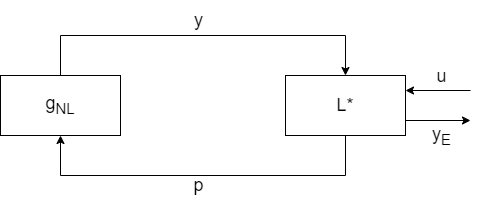
\includegraphics[scale=0.5]{figures/py.png}
    \caption{A rendszerből el lett távolítva a késleltetés nélküli rész; ebben a formában már nincs számítási probléma}
\end{figure}

\section{A K-módszer elemzése}\label{bilinearK}

Egy általános kauzális, idő-invariáns rendszernek az általános állapotváltozós leírása az alábbi alakban felírható~\cite{borin}\cite{borin2}\cite{otherK}:
\begin{subnumcases}{\label{avlna}} 
    \mathbf{\dot{w}}=\mathbf{Aw}+\mathbf{Bu}+\mathbf{Cy}\label{kw}\\
    \mathbf{x}=\mathbf{Dw}+\mathbf{Eu}+\mathbf{Fy}\label{kx}\\
    \mathbf{y}=\mathbf{f} (\mathbf{x})\label{ky}
\end{subnumcases}
ahol $w$ az állapotvektor és $u$ a bemenet.
Laplace-transzformálva, majd bilineáris transzformációt alkalmazva (\ref{kw}) egyenletre~\cite{borin}:
\begin{equation}
    s\mathbf{W(s)}=\mathbf{AW}(s)+\mathbf{BU}(s)+\mathbf{CY}(s)
\end{equation}
\begin{equation}
    h\frac{1-z^{-1}}{1+z^{-1}}\mathbf{W}(s)=\mathbf{AW}(s)+\mathbf{BU}(s)+\mathbf{CY}(s)
\end{equation}
ahol $h=\frac{2}{T}$. Ezt rendezve:
\begin{equation}
    h(1-z^{-1})\mathbf{W}(z)=\mathbf{A}(1+z^{-1})\mathbf{W}(z)+(1+z^{-1})(\mathbf{BU}(z)+\mathbf{CY}(z))
\end{equation}
\begin{equation}
    h\mathbf{W}(z)-\mathbf{AW}(z)=z^{-1}h\mathbf{W}(z)+z^{-1}\mathbf{AW}(z)+\mathbf{BU}(z)+\mathbf{CY}(Z)+z^{-1}(\mathbf{BU}(z)+\mathbf{CY}(z))
\end{equation}
\begin{equation}
    (h\mathbf{I}-\mathbf{A})\mathbf{W}(z)=z^{-1}(h\mathbf{I}+\mathbf{A})\mathbf{W}(z)+\mathbf{BU}(z)+z^{-1}\mathbf{BU}(z)+\mathbf{CY}(z)+z^{-1}\mathbf{CY}(z)
\end{equation}
Inverz z-transzformálva:
\begin{equation}
    (h\mathbf{I}-\mathbf{A})\mathbf{w}[n]=(h\mathbf{I}+\mathbf{A})\mathbf{w}[n-1]+\mathbf{Bu}[n]+\mathbf{Bu}[n-1]+\mathbf{Cy}[n]+\mathbf{Cy}[n-1]
\end{equation}
Ha ($h\mathbf{I}-\mathbf{A}$) invertálható (ami igaz lesz mindig, ha $h$ az $\mathbf{A}$ mátrix sajátértékeitől különbözik~\cite{borin}), akkor balról 
az inverzével beszorozva a két oldalt:
\begin{equation}
    \mathbf{w}[n]={(h\mathbf{I}-\mathbf{A})}^{-1}((h\mathbf{I}+\mathbf{A})\mathbf{w}[n-1]+\mathbf{Bu}[n]+\mathbf{Bu}[n-1]+\mathbf{Cy}[n]+\mathbf{Cy}[n-1])
\end{equation}
A könnyebb felírás érdekében új segédváltozók bevezetése ajánlott.
\begin{eqnarray}
    &\mathbf{G} \triangleq {(h\mathbf{I}-\mathbf{A})}^{-1}\mathbf{C}
   \label{G}\\
    &\mathbf{H} \triangleq {(h\mathbf{I}-\mathbf{A})}^{-1}(h\mathbf{I}+\mathbf{A})
   \label{H}\\
    &\mathbf{J} \triangleq {(h\mathbf{I}-\mathbf{A})}^{-1}\mathbf{B}
   \label{J}
\end{eqnarray}
Ezeket behelyettesítve:
\begin{equation}
    \mathbf{w}[n]=\mathbf{Hw}[n-1]+\mathbf{J}(\mathbf{u}[n]+\mathbf{u}[n-1])+\mathbf{Gy}[n-1]+\mathbf{Gy}[n]
\end{equation}
Egy újabb segédváltozó bevezetése:
\begin{eqnarray}
    \mathbf{\hat{p}} \triangleq \mathbf{Hw}[n-1]+\mathbf{J}(\mathbf{u}[n]+\mathbf{u}[n-1])+\mathbf{Gy}[n-1]
   \label{pk}
\end{eqnarray}
Ezt behelyettesítve:
\begin{equation}
    \mathbf{w}[n]=\mathbf{\hat{p}}[n]+\mathbf{Gy}[n]
   \label{wn}
\end{equation}
Az átalakítások segítségével a (\ref{kx}) egyenlet felírható:

\begin{equation}
    \mathbf{x}[n]=\mathbf{D\hat{p}}[n]+\mathbf{DGy}[n]+\mathbf{Eu}[n]+\mathbf{Fy}[n] = \mathbf{p}[n]+\mathbf{Ky}[n]
\end{equation}
ahol
\begin{equation}
    \mathbf{K} \triangleq \mathbf{DG}+\mathbf{F}
   \label{K}
\end{equation}
\begin{equation}
    \mathbf{p}[n] \triangleq \mathbf{D\hat{p}}[n]+\mathbf{Eu}[n]
\end{equation}

Összességében~\cite{borin}:
\begin{equation}
    \begin{cases}
        \mathbf{p}[n]=\mathbf{Hw}[n-1]+\mathbf{J}(\mathbf{u}[n]+\mathbf{u}[n-1])+\mathbf{Gy}[n-1]+\mathbf{Eu}[n] \\
        \mathbf{y}[n]=\mathbf{f}_{NL}(\mathbf{p}[n]+\mathbf{Ky}[n]) \\
        \mathbf{w}[n]=\mathbf{Hw}[n-1]+\mathbf{J}(\mathbf{u}[n]+\mathbf{u}[n-1])+\mathbf{Gy}[n-1]+\mathbf{Gy}[n]
    \end{cases}
   \label{keq}
\end{equation}
A (\ref{keq}) egyenletrendszerben az egyetlen problémát okozó rész a második egyenlet. 
Ezen kívül az egyenletrendszeren sorba iterálva minden elem kiszámolható, hiszen a $\mathbf{p}[n]$ 
csak a definiált és a múltbéli változóértékektől függ, a $\mathbf{w}[n]$ egyenletébe szintén csak be 
kell helyettesíteni az $\mathbf{y}[n]$ kiszámolása után.

Érdemes megjegyezni, hogy ezt a módszert másféle folytonos időből diszkrét időbe transzformációval 
is le lehet vezetni (például hátralépő Euler módszerrel)~\cite{borin}.

\section{A nemlineáris rész}
A korábbi fejezetben látható, hogy a számítási problémát korlátozódik (\ref{keq}) második 
egyenletére:
\begin{equation}
    \mathbf{y}[n]=\mathbf{f}_{NL}(\mathbf{p}[n]+\mathbf{Ky}[n])
   \label{nonlineq}
\end{equation}
A cél az egyenletek rendezésével az volt, hogy olyan formára legyen hozva a megoldandó számítási 
problémát okozó egyenlet, hogy arra alkalmazható legyen a Dini-tételt.
\subsection{Dini-tétel}\label{dini}
A Dini-tételnek csak a SISO rendszerekre vonatkoztatott alakját tárgyalja ez a dokumentum (MISO és 
MIMO rendszerekre is meg lehet fogalmazni~\cite{borin}). Adott egy implicit függvény: 
\begin{equation}
    f(x,y)=0
\end{equation}
Ha ennek a függvénynek létezik olyan pontja, amelyre igaz egy $P_0(x_0, y_0)$ pontban, hogy
\begin{equation}
    \frac{\partial{f}}{\partial{y}}\biggr |_{(x_0, y_0)} \neq 0
   \label{partial}
\end{equation}
akkor létezik olyan $g(x)$ függvény, amelyre
\begin{equation}
    f(x, g(x))=0
\end{equation}
igaz a $P_0$ pont körül. Könnyen belátható, hogy (\ref{partial}) nem csak $P_0$-ra, hanem az egész 
$f(x,y)$ függvényre igaz, akkor $f(x,y)$ nem csak lokálisan, hanem globálisan is kifejezhető 
$f_{NL}(x,g(x))$ függvénnyel~\cite{borin}.

Ebben az esetben az $f(x,y)$ függvény a (\ref{nonlineq}) nullára rendezett alakja:
\begin{equation}
    f_{NL}(p+ky)-y=0
\end{equation}
Ha az y szerinti parciális deriváltjára adott a feltétel, azaz
\begin{equation}
    \frac{\partial{f}}{\partial{y}}=f'_{NL}(p+ky)k-1 \neq 0
\end{equation}
\begin{equation}
    f'_{NL}(p+ky) \neq \frac{1}{k}
\end{equation}
akkor létezik $g(p)$, amelyre
\begin{equation}
    g(p)=y
\end{equation}
Mivel ismerjük az $f(x)=y$ függvényt, ezért geometriai megfontolások 
miatt~\cite{borin} a $g(p)$ függvényt az $f(x)$ függvény lineáris transzformációjával 
kapható meg, mégpedig a
\begin{equation}
    \begin{cases}
        y=y_s \\
        p=x-ky
    \end{cases}
\end{equation}
lineáris transzformáció segítségével, ami az $(x,y)$ síkból a $(p,y_s)$ síkba transzformál.

\section{A K-módszer alkalmazása}
A korábban már levezetett (\ref{keq}) szerint:
\begin{equation}
    \begin{cases}
        \mathbf{p}[n]=\mathbf{Hw}[n-1]+\mathbf{J}(\mathbf{u}[n]+\mathbf{u}[n-1])+\mathbf{G}\mathbf{y}[n-1]+\mathbf{Eu}[n] \\
        \mathbf{y}[n]=\mathbf{f}_{NL}(\mathbf{p}[n]+\mathbf{Ky}[n]) \\
        \mathbf{w}[n]=\mathbf{Hw}[n-1]+\mathbf{J}(\mathbf{u}[n]+\mathbf{u}[n-1])+\mathbf{Gy}[n-1]+\mathbf{Gy}[n]
    \end{cases}
\end{equation}
Ha ez az egyenletrendszert a korábban bevezetett változók szerint kerül felírásra, akkor ezeken 
végigiterálva a nemlineáris rendszer egyenleteinek megoldása lesz az eredmény~\cite{borin}.
\begin{equation}
    \begin{cases}
        \mathbf{\hat{p}}[n]=\mathbf{Hw}[n-1]+\mathbf{J}(\mathbf{u}[n]+\mathbf{u}[n-1])+\mathbf{Gy}[n-1] \\
        \mathbf{p}[n]=\mathbf{D\hat{p}}[n]+\mathbf{Eu}[n] \\
        \mathbf{y}[n]=\mathbf{g}(\mathbf{p}[n]) \\
        \mathbf{w}[n]=\mathbf{Gy}[n]+\mathbf{\hat{p}}[n]
    \end{cases}
   \label{iter}
\end{equation}
A (\ref{iter}) egyenletrendszer harmadik egyenlete megoldható például egy előre legenerált 
táblázat szerint, amiben az $(p,y)$ értékpárokat tároljuk le, és ezek közül lesznek az értékpárok kikeresve. 
Ez a rész fogja a K-módszer hatékonyságát adni, hiszen így nem valós időben kell egy 
implicit egyenletrendszert megoldani, hanem egy előre legenerált táblázatból elég kikeresni 
az eredményt.\\
Összefoglalva az algoritmus lépéseit~\cite{otherK}:
\begin{enumerate}
    \item $\mathbf{\hat{p}}[n]$ kiszámolása (\ref{pk}) szerint
    \item $\mathbf{p[n]}$ kiszámítása $\mathbf{\hat{p}}[n]$ és $\mathbf{u}[n]$ felhasználásával
    \item $\mathbf{y[n]}$ kiszámítása a letárolt táblázatban való kereséssel
    \item Az állapotáltozók ($\mathbf{w}$) frissítése (\ref{wn}) szerint
    \item A kimenet kiszámolása $\mathbf{w}[n]$, $\mathbf{u}[n]$, $\mathbf{y}[n]$ segítségével
\end{enumerate}

\section{Példa}
A módszer bemutatása céljából a Tube-Screamer áramkörének a ``clipping stage``részét valósítottam meg K-módszer segítségével. 

\begin{figure}[H]
    \centering
    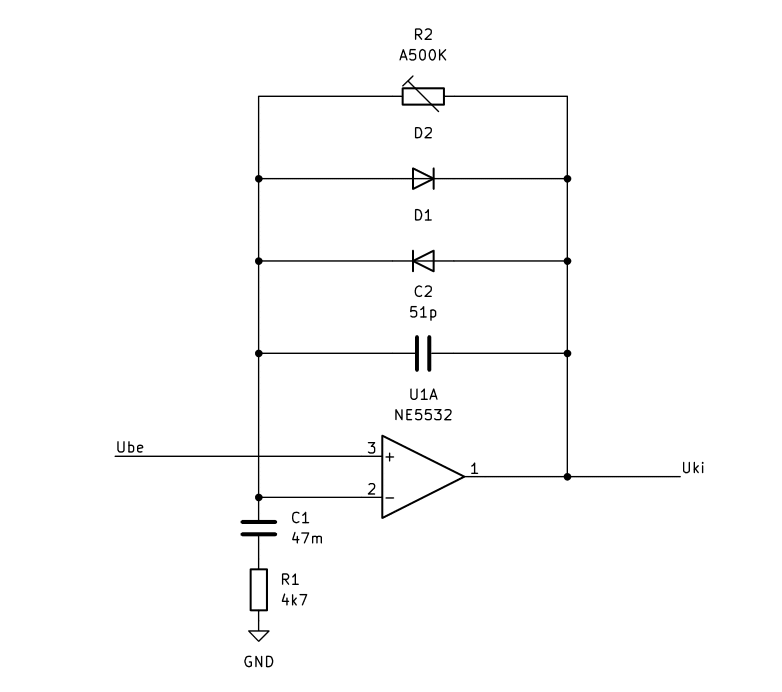
\includegraphics[scale=0.9]{figures/TSCS.png}
    \caption{A Tube-Screamer áramkör ``clipping stage``részének áramköre}
\end{figure}

\subsection{Megvalósítás}
Először meg kell határozni a rendszer állapotváltozós leírását. Az állapotváltozóknak a kondenzátorok 
feszültségét veszem fel. A diódákat összevonom, és egy nemlineáris elemként kezelem. A nemlineáris 
függvény pedig a két diódakarakterisztika összege lesz. A Kirchoff-törvényekből felírt egyenleteket 
átrendezve:
\begin{equation}
    \begin{cases}
        u_{C1}'=-\frac{1}{R_1C_1}u_{C1}+\frac{1}{R_1C_1}u_{be} \\
        u_{C2}'=-\frac{1}{C_2R_1}u_{C1}-\frac{1}{C_2R_2}u_{C2}+\frac{1}{C2R1}u_{be}-\frac{1}{C_2}f(u_{C2}) \\
        f(u)=I_{S0}(e^{\frac{u}{u_T}}-e^{\frac{-u}{u_T}}) \\
        u_{ki}=u_{C2}+u_{be}         
    \end{cases}
   \label{diodak}
\end{equation}
A K-módszerhez szükséges mátrix alakban felírva:
\begin{equation}
    \begin{cases}
        \mathbf{\dot{w}}=
    \begin{pmatrix}
        -\frac{1}{R_1C_1} & 0 \\
        -\frac{1}{C_2R_1} & -\frac{1}{C_2R_2}
    \end{pmatrix}
    \mathbf{w}+
    \begin{pmatrix}
        \frac{1}{R_1C_1} \\
        \frac{1}{C2R1}
    \end{pmatrix}
    u+
    \begin{pmatrix}
        0 \\
        -\frac{1}{C_2}
    \end{pmatrix}
    y \\
    x=
    \begin{pmatrix}
        0 & 1
    \end{pmatrix}
    w \\
    y=f(x)
    \end{cases}
\end{equation}
Az ebből meghatározott mátrixok:
\begin{equation}
    \begin{array}{c}
        \mathbf{A}=
    \begin{pmatrix}
        -\frac{1}{R_1C_1} & 0 \\
        -\frac{1}{C_2R_1} & -\frac{1}{C_2R_2}
    \end{pmatrix}
\quad  
\mathbf{B}=
    \begin{pmatrix}
        -\frac{1}{R_1C_1} & 0 \\
        -\frac{1}{C_2R_1} & -\frac{1}{C_2R_2}
    \end{pmatrix}
\quad 
\mathbf{C}=
    \begin{pmatrix}
        0 \\
        -\frac{1}{C_2}
    \end{pmatrix} \\ 
    \\ 
    \mathbf{D}=
    \begin{pmatrix}
        0 & 1
    \end{pmatrix}
\quad  E=0\quad F=0
    \end{array}
\end{equation}
A segédváltozókat kiszámolom a (\ref{G}), (\ref{H}), (\ref{J}), (\ref{K}) egyenletekkel. 

Legenerálom az $f(u)$ függvény táblázatát, majd végrehajtom rajta az $y_s=y$, 
$p=x-Ky$  lineáris transzformációt. Lehetőség szerint érdemes csak a valóságban is előforduló 
két szélsőérték határán belüli értékeket legenerálni, illetve ha az $y$ tengelyre szimmetrikus a függvényünk, 
akkor csak az egyik oldalt letárolni (ennél a példánál ez pont lehetséges).
Ezután már csak futtatni kell a (\ref{iter}) pontban leírt algoritmust.

\subsection{Eredmény}
Az áramkört az LTSpice programban is elkészítettem összehasonlítás céljából, és teszteltem a K-módszert 
a fent említett függvénnyel, illetve LTSpice-ból kiexportált karakterisztikával.

\begin{figure}[!h]
    \centering
    \begin{subfigure}{0.47\textwidth}
        \centering
        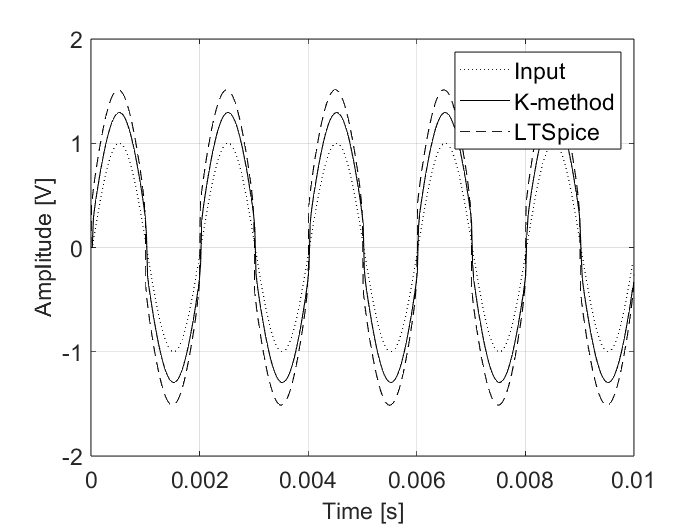
\includegraphics[scale=0.38]{figures/ownmodel.png}
        \caption{A (\ref{diodak}) egyenletben leírt karakterisztikával}\label{a}
    \end{subfigure}
    \hfill
    \begin{subfigure}{0.47\textwidth}
        \centering
        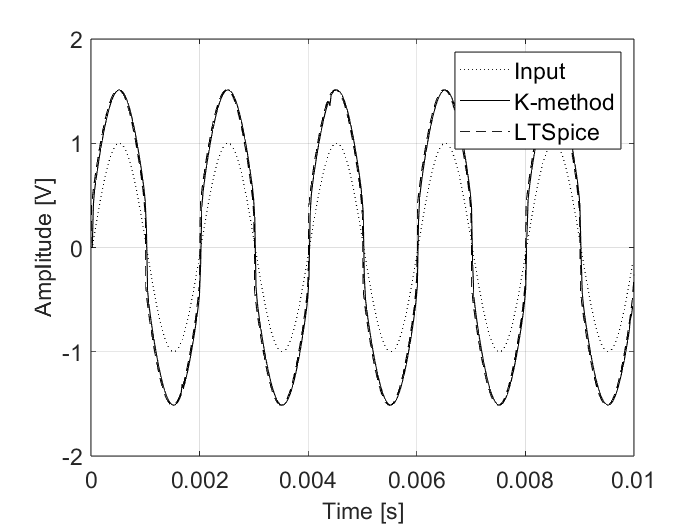
\includegraphics[scale=0.38]{figures/spicemodel.png}
        \caption{LTSpice-ból exportált karakterisztikával}\label{b}
    \end{subfigure}
    \caption{A megvalósított modell válaszjele egy $500 Hz$ frekvenciájú, $1 V$ amplitúdójú szinusz 
    jelre}
\end{figure}
A (\ref{diodak}) egyenletrendszerben említett karakterisztikával az eredmény eltér az LTSpice program által 
meghatározott kimenettől, ami a (\ref{a}) ábrán látható. A jelalakok hasonlóak, viszont amplitúdóban különböznek. Ez 
azért van, mert az LTSpice nem ugyan ezzel a karakterisztikával számol. Erre abból lehet következtetni, hogy 
ha az LTSpice-ból exportáljuk a karakterisztikánkat, akkor a kimenetek megegyezőek lesznek, ahogy látható a (\ref{b}) ábrán is.